% \subsection{Problem Formulation}

We consider a probabilistic approach to trajectory forecasting. Ideally, we want the predicted distribution to be both sharp and valid under the definition in \Eqref{eq:coverage}. To quantify the uncertainty, we review the classic score function Mean Interval Score (MIS) and derive a 2 dimensional extension, Mean Regional Score (MRS).

% \leo{Is 'interval' a proper terminology here? Empirically it's a 1-d concept, for n-d interval people always mean region with square bounding. It's confusing especially when the mean interval score below is a 1-d metric.} 

% For each agent in the scene, we estimate a sequence of $k$ prediction regions $\Hat{C}_{t+1:t+k}$ for $\mathbf{x}_{t+1:t+k}$. The intervals $\Hat{C}$ are dependent on a significance level $\alpha$, denoted  as $\Hat{C}^{\alpha}$. 

% given by $p_\theta( \mathbf{x}_{t+1:t+k} | \mathbf{x}_{1:t}, \mathbf{e})$,


\paragraph{Mean Interval Score.}
Mean Interval Score (MIS) is a proper scoring rule \cite{properscoring} for interval forecasts that rewards narrower confidence intervals and encourages coverage. 
%
Specifically, let $Y  \sim {P}_Y$ be a one-dimensional random variable, and an upper bound $u$, a lower bound $l$ be its estimated $\frac{\alpha}{2}$ and $(1-\frac{\alpha}{2})$ quantiles respectively, MIS is defined using samples $y_i \sim {P}_Y$.
 %
\begin{align}
    \mathrm{MIS}(u,l; Y) = \frac{1}{N} \sum_{i=1}^{N}[(u-l) +
     \frac{2}{\alpha}(y_i-u)\mathbb{1}\{y_i>u\}\nonumber 
     + \frac{2}{\alpha}(l-y_i)\mathbb{1}\{y_i<l\} ] 
    \label{eq:mis}
\end{align}
%
Where the three terms in  \Eqref{eq:mis} accounts for the width of the interval, and how much the sample point exceeds the upper bound and the lower bound, respectively. MIS has the advantage of being easy to compute and does not require the model to be parametric \cite{properscoring}. It can also be used as an objective function for probabilistic forecasting \cite{wu2021quantifying}. 


\paragraph{Mean Regional Score.}
For n-D distributions, we introduce a new metric called the Mean Region Score (MRS), which generalizes MIS to higher dimensions. 
%
Let $Z \sim {P}_Z$ be an n-dimensional continuous random variable. First, we need to generalize  $\alpha$-quantile and define the  confidence region. Let the region bordering $z$ as $R(z)$, the  confidence region of level $\alpha$ 
\begin{align}
R_P(\alpha) =  \inf \lbrace R(z)  | \int_{R(z)} P( z ) dz \geq \alpha \rbrace
\end{align}
is the smallest region whose probability exceeds  level $\alpha$.

\begin{figure}
    \centering
  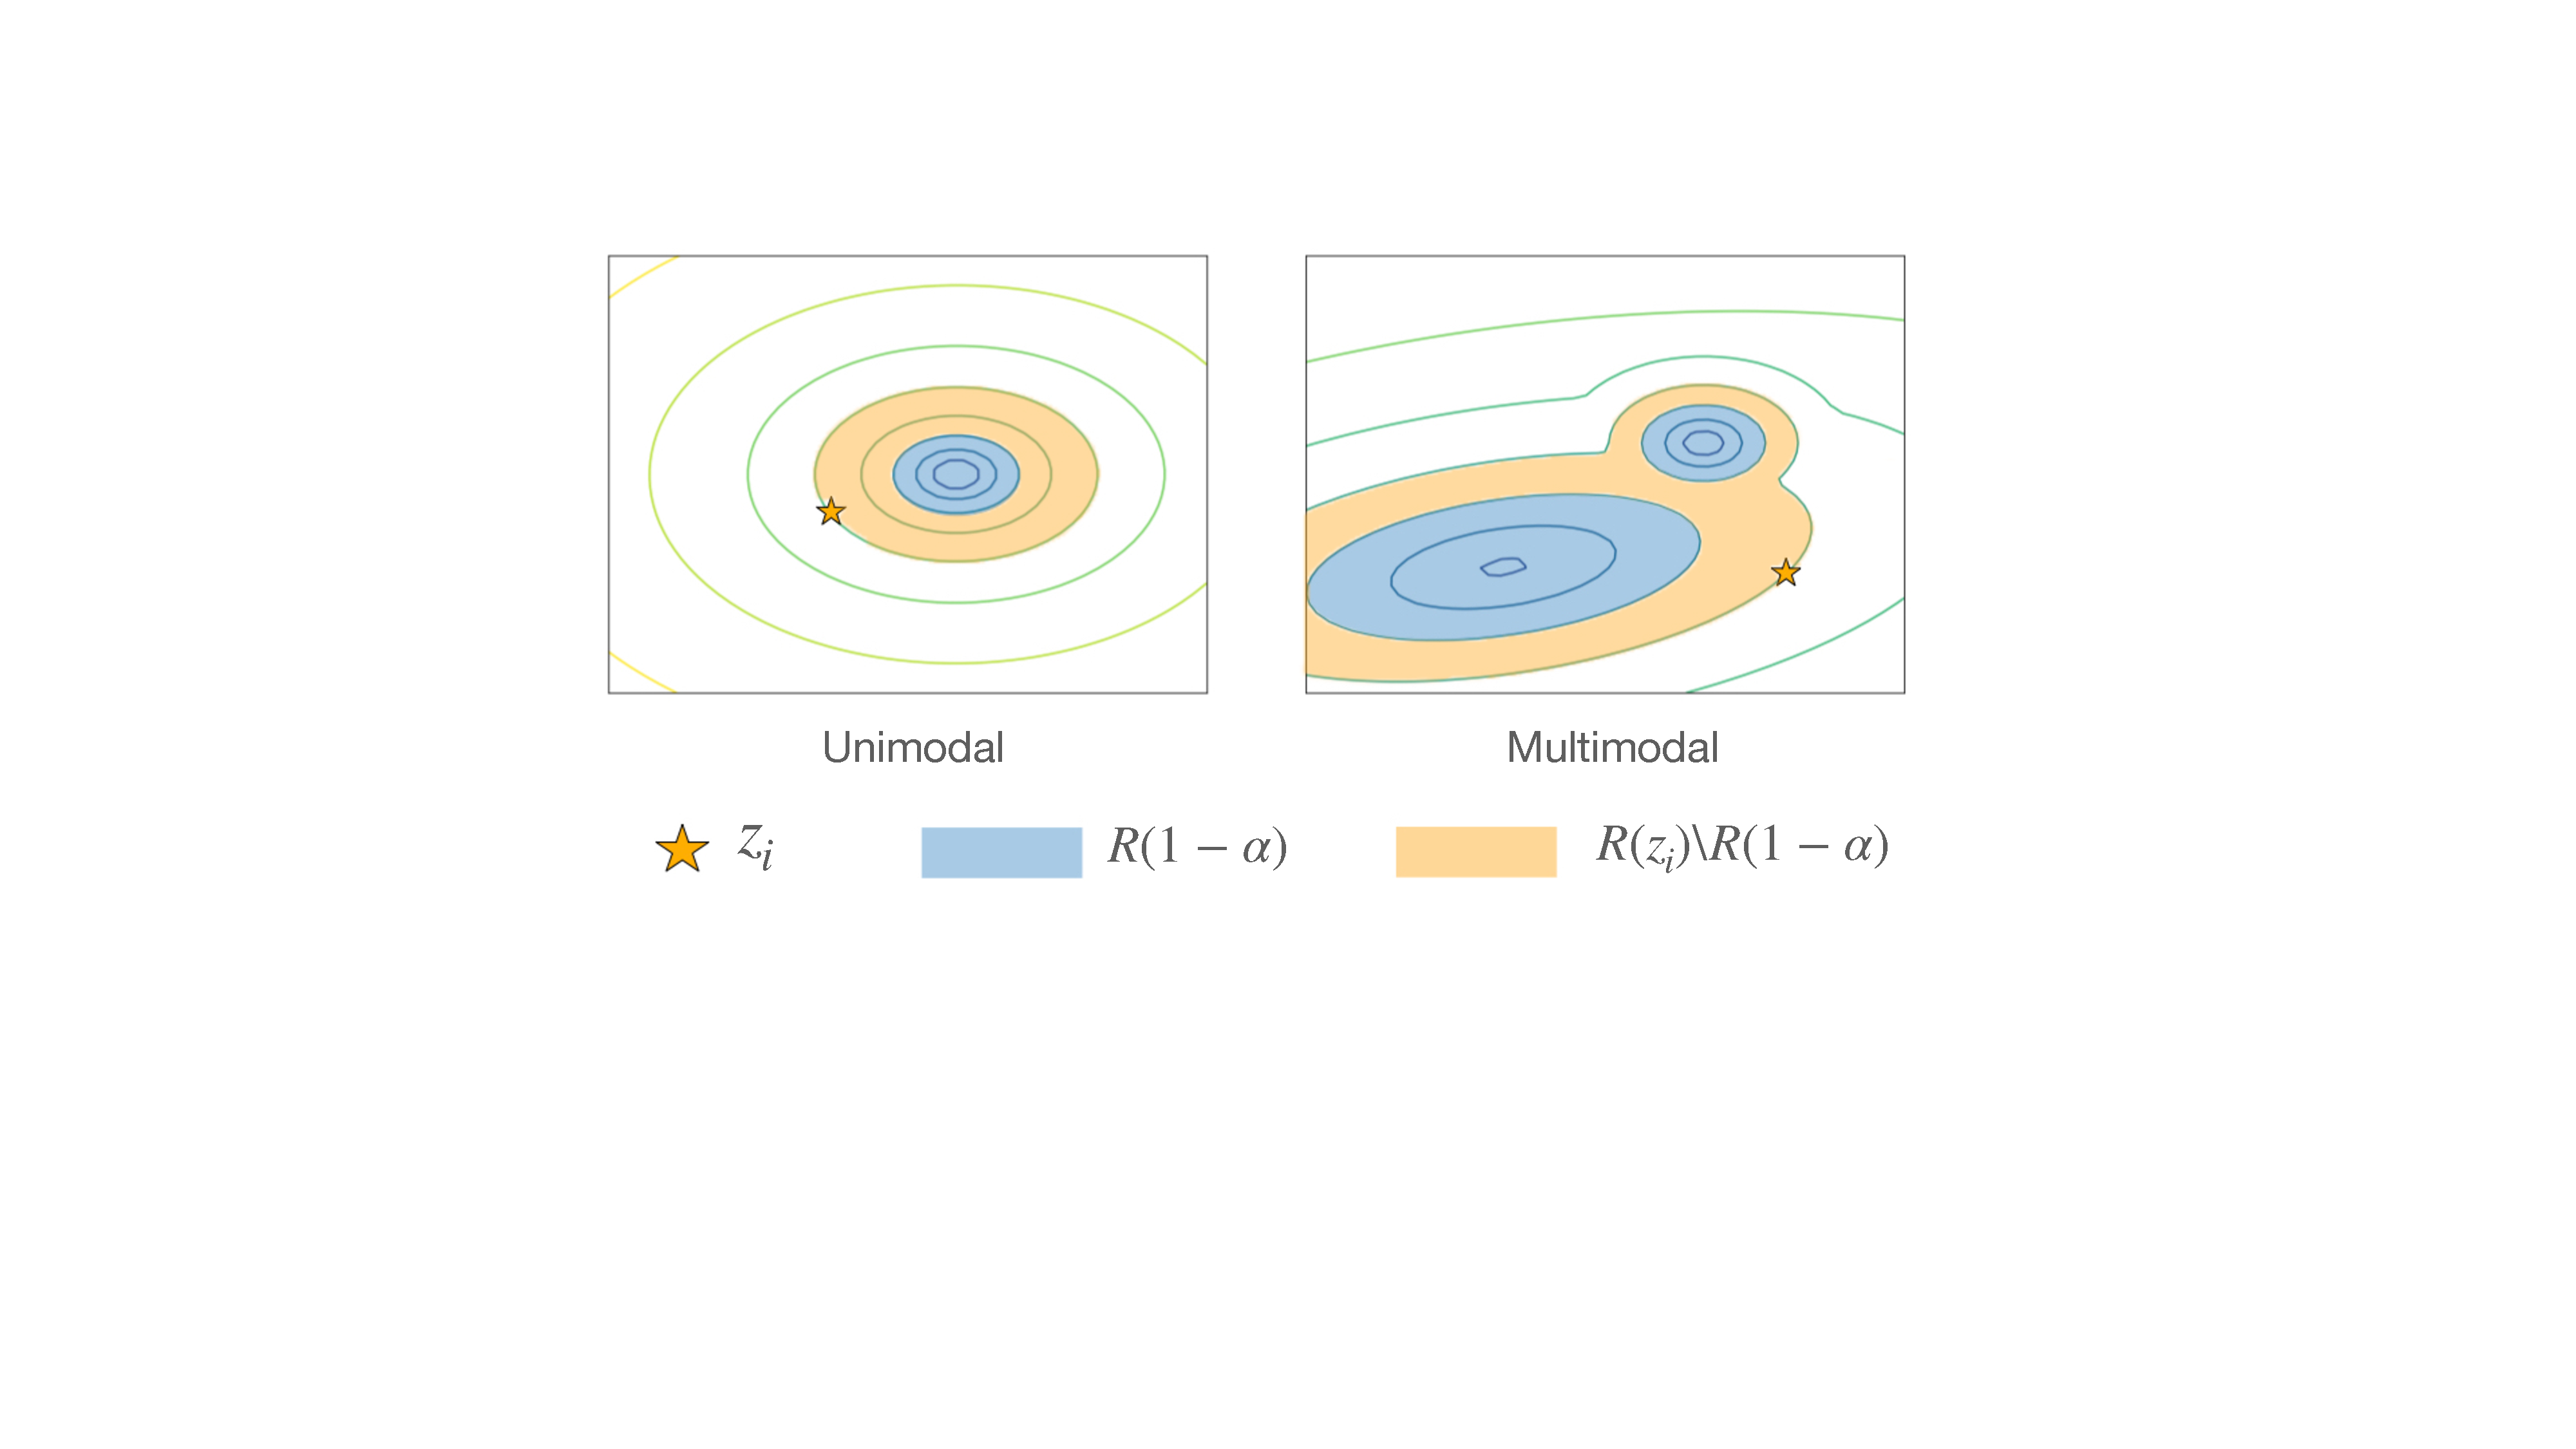
\includegraphics[width=.8\linewidth]{equivariance/figs/mrs.pdf}
  \caption{MRS illustration for   unimodal and multimodal distributions. Given a sample $z_i$, MRS  calculates the area of blue region plus that of the the orange region scaled by $1/\alpha$. }
  \label{fig:mrs}
\end{figure}
When the distribution is Gaussian $P_Z =\mathcal{N}(\mu, \Sigma)$ with mean $\mu \in \mathbb{R}^n$ and the covariance matrix $\Sigma \in \mathbb{R}^{2\times 2}$ that is positive definite. The $(1-\alpha)$ confidence region of an n-D multivariate normal distribution $P = \mathcal{N}(\mu, \Sigma)$ is an ellipsoid that can be written as \cite{slotani1964tolerance}:
\[
    R(1-\alpha) = \{ z| (z-\mu)^T \Sigma^{-1} (z-\mu) \leq  \chi_n^2(1-\alpha)\}.
\]
where $\chi_n^2$ is the chi-squared distribution with n degrees of freedom.
Then, for a given sample $z_i \in \mathbb{R}^n$, we can draw an ellipsoid whose edge coincides $z_i$ defined as 
\[
    R(z_i) = \{z|(z-\mu)^T\Sigma^{-1}(z-\mu) \leq c'\} 
\]
where $c' = (z_i - \mu)^T \Sigma^{-1} (z_i - \mu)$.


% The smallest confidence region of  $1-\alpha$ could be viewed as a superlevel set of points with probability greater than a threshold $\zeta_{1-\alpha}$. \cite{multimodalconfidence}




The MRS score of the $(1-\alpha)$ prediction interval thus can be evaluated as:
%
\begin{align}
    \mathrm{MRS}(R ;Z) = \frac{1}{N} \sum_{i=1}^N  [|R(1-\alpha)| +   \frac{1}{\alpha}| R(z_i) \backslash R(1-\alpha)| \mathbb{1} \{z_i \in R^C(1-\alpha)\}]
\label{eq:mrs}
\end{align}
where the first term  corresponds to the area of the confidence region and the second term measures how much each data $z_i$ deviates from the region. $|\cdot|$ measures the size of the set.  It is also easy to prove (see Appendix \ref{app:properscoring}) that MRS is a proper scoring rule \cite{properscoring}, which means MRS is optimized if and only if the distribution $P$ recovers that of $Z$.

Figure \ref{fig:mrs} illustrates MRS for both unimodal and multimodal distributions.  Note that when the distribution is single-modal, the confidence interval in \Eqref{eq:mrs} is both \textit{equally tailed} and the \textit{shortest} confidence interval. For  multi-modal distributions,  we solve for the \textit{smallest} confidence region to cover probable events. In appendix \ref{app:mrsgeneral} we present a method to estimate MRS for arbitrary 2-D distributions, where we divide the domain space into small grids to estimate density, and obtain $R(1-\alpha)$ and $R(z_i)$ by assembling high density regions.
%


%For an arbitrary distribution $P$ over $\mathbb{R}^2$, we can define the confidence region $S_P$ as the superlevel set $S_P(1-\alpha) = \lbrace x \in \mathbb{R}^2 | p(x) \geq c(\alpha) \rbrace$, where $c(\alpha)$ is defined such that 